\documentclass[12pt]{report}
\usepackage[utf8]{inputenc}
\usepackage{graphicx}
\usepackage[tmargin=2cm, lmargin=4cm, rmargin=2.5cm, bmargin=4cm, paperwidth=8.267in, paperheight=11.692in]{geometry}
\usepackage{amsfonts}
\usepackage{array}
\usepackage{indentfirst}
\graphicspath{ {images/} }
\usepackage{lipsum}
\usepackage{verbatim}
\usepackage{titlepic}
\usepackage{amsmath}
%\usepackage{titlesec}

\begin{document}

\title{Light Field Research \vspace{2.5cm}}	%
\includegraphics[scale=0.2]{university_edinburgh.jpg}
\author{
\Large Carson Vogt \vspace{1cm} \\ 
}

\date{
	\centering
	PhD \endgraf\medskip
	Heriot-Watt University \endgraf\medskip
	31 August 2015
}

\maketitle

\begin{abstract}
\begin{small}
abstract
\end{small}
\end{abstract}

\listoffigures

\tableofcontents

\chapter*{Introduction}
What is your hypothesis

"There are many potential formats which could be used for VR video.
Lightfields [Levoy and Hanrahan 1996] provide the greatest level of
immersion if they can be captured for a suitable volume"

"...a practical solution for this has not yet been demonstrated"

Current light field technology is built on the parameterization put forward by Levoy in 1996. If we go back just five years to the original paper regarding the plenoptic function, we see a critical element missing from the the function: time. There are a number of major limitations associated with light fields. For one, the method for data collection is often bulky or slow and extremely limited in its capabilities (cite the papers). Up until recently, it has required a static scene, but advances in light field cameras and processing power have seen small advancements in light field video (cite). Regardless, this still leaves the user with the first problem. Another issue is the lack of mobility within a scene and capture. With current rendering techniques, the parameterization is adhered to exactly. That is to say, if image capture is done two dimensionally, it must remain so. 

We aim to not only improve on the work of (unstructured light fields), but to develop a system that can take time into account for a dynamic light field experience. 

Light fields are a rising method for rendering scenes. With the rising popularity of virtual reality, light field technology has the potential to revolutionize the way in which viewers interact with subjects of interest, like sports matches.

WE want to create a system that can capture a light field and effectively turn it back into a 5D problem, where time is one of the specified parameters

Given a set of discrete samples (complete or incomplete), from the plenoptic function, the goal of image-based rendering is to generate a continuous representation of that function\cite{McMillan95}

\chapter*{Literature Review}
The light field is, at its base, a derivation of the plenoptic function (the root \emph{plenus} meaning complete, and optic). The plenoptic function, the concept for which was set forward by Adelson and Bergen in 1991, is a method of mathematically describing the elements of vision. The paper takes on the daunting task of defining what can be seen across 3D space, where every point (or pencil of rays) contains the information for all of the rays passing through it.  This is illustrated well in figure  \ref{fig:plenoptic_visual}. 
\begin{figure}[!ht]
	\centering
	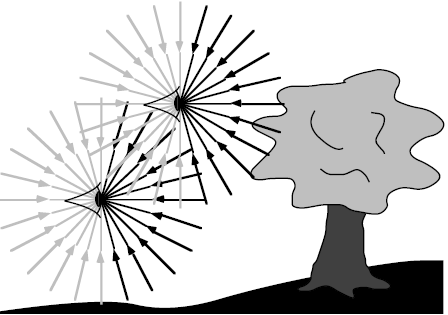
\includegraphics[scale=0.75]{plenoptic_image.png}
	\caption{The plenoptic function sampled at two points, showing all pencils of light rays which pass through those points \cite{Adelson91}.}
	\label{fig:plenoptic_visual}
\end{figure}
The concept of all light passing through a point is rooted in the early observations of Leonardo da Vinci, who observes the effect of a hole in a wall, which reveals an image of the scene in front of the wall, upside down on the back wall \cite{Adelson91}. This is the concept behind the pinhole camera, which is a key assumption applied to cameras in much of the work done with light fields. The next section reviews the derivation of the 4D light field from the 7D plenoptic function.  

\section*{Early Research and Derivation from Plenoptic Function}
Having a basic idea of what constitutes light in space, Adelson and Bergen set forth to mathematically represent this plenoptic function.
The function itself is given as 
\begin{equation}
P=P(\theta,\phi,\lambda,t,V_x, V_y,V_z)
\end{equation}
where $\theta$ and $\phi$ are the viewing angles from a point in space, $\lambda$ ***mention radiance*** is wavelength of the incoming ray, $t$ is the time parameter at which the ray is observed, and $V_x,V_y,V_z$ define the location in three dimensional space \cite{Adelson91}. This defines the incoming rays at every point in 3D space for all time, which would theoretically allow for the reconstruction of any view. Measuring the plenoptic function comes with its own set of difficulties though.

In \cite{McMillan95} and \cite{Huang14}, the 7D plenoptic function is reduced to five dimensions,
\begin{equation}
p=P(\theta,\phi,V_x,V_y,V_z)
\end{equation}
where $t$ and $\lambda$ are omitted as the time of sampling is considered to be constant (therefore requiring the scene remain static) and the radiance is*** (Look in Levoy06a). 

In Levoy and Hanrahan's seminal paper \emph{Light Field Rendering} \cite{Levoy96}, the authors note that in space free of occlusions, the function can be further reduced to a four dimensional function as the ray of light reaching the pixel will not be altered in free space. In this environment, the only requirement is to know the direction of a ray, which is a function of four points shown in the following equation:
\begin{equation}
r=L(u,v,s,t)
\end{equation}
where $r$ is the individual ray passing through the planes. This parameterization requires a ray to pass through two known planes, defined as the $s,t$ and $u,v$ planes. This is  still a standard parameterization, used in \cite{Isaksen01}, \cite{Vaish06}, and \cite{Oberlin16}, among others. In one case, a three dimensional parameterization is used as acquisition is completed by using a 1D row of cameras \cite{Kim13}. Levoy and Hanrahan introduce the two plane parameterization as the light field \cite{Levoy96}.

While \cite{Levoy96} introduces the popular two plane parameterization, McMillan and Bishop define a cylindrical parametrization a year earlier. Having encountered difficulties storing a spherical parameterization on a computer, the authors note that with a cylinder, it can effectively be unrolled into a plane, thus making it easy to store and access \cite{McMillan95}.

For non-synthetic rendering systems.

Rendering may be viewed as a reconstruction
of the light field forming an estimate of the
perceived image around the objects
(Kriging Paper)

In \emph{Light Fields and Computational Imaging}, Levoy outlines the available parameterizations as of 2006, shown in figure \ref{fig:parameterization_visual}
\begin{figure}[!ht]
	\centering
	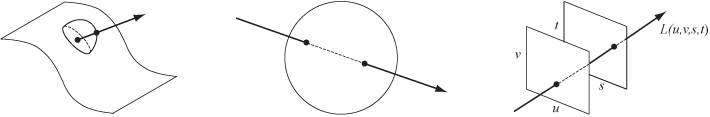
\includegraphics[scale=0.75]{Light-field-parameterizations.png}
	\caption{The plenoptic function at two points, showing all pencils of light rays \cite{Adelson91}}
	\label{fig:parameterization_visual}
\end{figure}

With Isaksen \emph{et al}'s \emph{Dynamically Reparameterized Light Fields}

LIGHT FIELD EFFECTS
Learning Based View Synthesis


\section*{Light Field Collection}
While light field collection has gone relatively unchanged through the years, there are some interested new approaches to collection, but they are still underdeveloped at this stage. 

The primary method by which light fields are captured is a brute force method relying on a large array of cameras \cite{Ng06}**** or a robotic gantry set to move to specific locations, thereby mimicing the camera array. These can be done as the parameterization used ignores the time component of the 7D plenoptic function. While a number of groups have shown interesting use cases for the camera array (some of which will be covered in later sections) such as \cite{Ng06}*****, it is not a practical method for capturing difficult scenes.

Utilizing the growing capabilities of image sensors, Ng shows in his thesis a way by which a light field can be captured by a single camera. Rather than producing a single image, a microlens array is inserted into the camera, after the lens and before the image sensor (see figure). This enables the user to create such effects as refocusing and some minimal movement around the image for a 3D effect after the image has been captured \cite{Ng06}. The light field camera still suffers from a lack of **spatial and angular resolution, leaving room for research to be done combining the light field camera and novel collection techniques.

Another unique data collection method was demonstrated in Davis \emph{et al's} paper, \emph{Unstructured Light Fields} from 2012 \cite{Davis12}. In it, Davis 

Minimizing the amount required to collect(cite review and actual article)
Move on to the more recent papers of Sparse lightfields and learning 
based view synthesis

Unstructured light fields paper also shows a method for collection utilizing a single camera and a SLAM algorithm known as PTAM(cite PTAM paper). Of course, this research is now a bit aged and can be improved in a number of ways, potentially expanding it significantly with the addition of a more robust and wide-ranging(?) SLAM method such as ORB-SLAM2(cite)

\cite{Ng06}
\cite{Davis12}
\cite{Oberlin16}


While light field rendering is the most immersive image-based rendering technique, one of the drawbacks of the light field is that the number of images required to create a high resolution and immersive scene can be prohibitively large \cite{Anderson16}. This leads to the natural question of the amount of sampling required for a complete or usable light field. There's surprisingly limited number of papers on the subject, which likely has to do with the methods for data collection, and thus it is one of the less-studied areas within the light field field.

\subsection*{Images Required}

\cite{Levoy06a} cites several papers which mention the requirements for obtaining a full light field using pre-2006 techniques. 

Chai \emph{et al} sets about to describe a formula which described the distance between sampling cameras \cite{Chai00}.

\cite{Isaksen01} mentions it how?

In Gortler***s paper, \emph{The Lumigraph}, it is noted that fewer images are required if the collector has some knowledge of the geometry of the scene \cite{Gortler96}. This concept is also made use of in more recent papers, such as \cite{Kim13}

One of the less studied areas is the amount of data required for a quality light field.
In \cite{Levoy06a}, Levoy briefly covers the amount of data required for an effective and high quality light field (Insert a quote here).

The subject had been previously covered first in \cite{Gortler96} then in \cite{Isaksen01} and \cite{Chai00}
In \cite{Shi14}, by analyzing the sparsity in the continuous Fourier domain, show that if light fields are collected to optimize for this, the number of images required to create a light field may be drastically reduced, 
\section*{View Creation}
The most heavily studied area with light fields is on the methods used for creating new images given missing, sparsely sampled light fields or ***

In \emph{Light Field Rendering}, Levoy and Hanrahan outline what would become the baseline for rendering views from a large set of collected images using the parameterization described in the previous section. 
\cite{Katayama95} Viewpoint dependent stereoscopic display
\cite{Kim13} scene reconstruction

In \emph{Light Field Reconstruction Using Sparsity in the Continuous Fourier Domain}, the authors show that light fields are sparse in the continuous Fourier domain \cite{Shi14} 

In one of the most recent papers on the subject, Kalantari \emph{et al}, rather than examine light fields in the Fourier domain, they train convolutional neural networks on new view synthesis within light field cameras. Their results suggest that their method, at least on the small scale of a light field camera, produces superior images compared with the previous state of the art \cite{Kalantari16}. Potential future work might be applying this to light fields with lower spatial and angular resolution that might have been collected by robots.

\cite{Ihrke16} Principles of light field imaging

\section*{Application of Light Fields}
Graphics and virtual reality are the most obvious applications for light fields and have effectively spurred on the field since the middle of the 1990s. Light fields are ve and realistic.

\begin{figure}[!ht]
	\centering
	\begin{minipage}{0.45\textwidth}
		\centering
		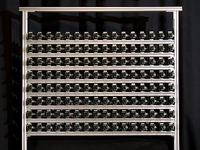
\includegraphics[scale=0.9]{stanford_camera_array.png}
		\caption{The dense camera array used at Stanford to capture a number of light fields.}
		\label{fig:camera_array}
	\end{minipage}\hfill
	\begin{minipage}{0.45\textwidth}
		\centering
		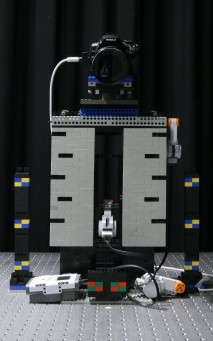
\includegraphics[scale=0.5]{lego_gantry.jpg}
		\caption{Another collection method, the gantry effectively mimics the camera array so long as the scene is not altered between gantry locations.}
		\label{fig:lego_gantry}
	\end{minipage}
\end{figure}

Riding on the work of Ng and the light field camera, Levoy \emph{et al} struck again with a paper on light field microscopy.\cite{Levoy06b}

In \cite{Vaish06} Vaish \emph{et al} utilize a large camera array to Demonstrate a method by which occlusions can effectively be removed if the light field is sampled densely enough, comparing several different techniques.

Some research has been done in light field videography, but it has been largely untouched. Wilburn \emph{et al}, utilizing a dense camera array, create a method for creating a high framerate system. However, the large camera array comes with its own set of problems in the form of.. It is not until 2016 that Google in a paper by Anderson \emph{et al} demonstrated effective light field video, bringing the generally left out time dimension back into the parameterization \cite{Anderson16}. 

It was Davis \emph{et al} who attempted to bring light fields to a consumer level outside of the light field camera concept put forward by Ng. While the use cases are limited, they went as far as developing an app that allowed users to capture their own light field and extract subjects from it as 3D objects \cite{Davis12}. Using a spherical parameterization, Davis \emph{et al} construct a light field by guiding a user with a graphical user interface that instructs the user on where to hold the camera for data collection.

Working at about the same time as Davis \emph{et al}, Jachnik \emph{et al} create a very similar system. While there are differences in user interface, and algorithmic difference, the concept is quite similar. However, after capturing a light field, the authors attempt to create a crude environment map, and from that the locations of light sources. The results are unique in that for augmented reality applications, shadowing can be implemented on an object that has been placed into a scene, creating a greater sense of realism \cite{Jachnik13}.

\section*{Future Collection Methods}
With a few exceptions, the direction of light field capture has largely been constant with researchers relying on the large camera array depicted in figure*** While there have been other methods, such as those of Ng, Davis \emph{et al}, and Jachnik \emph{et al}, they are either limited in their spatial and angular representations, or require significant human interaction to actually create the light field.

 \cite{Oberlin16} demonstrated the ability to caputure a light field with a seven degree of freedom robot arm on a Baxter robot. While there is no doubt that this is a definite move from traditional collection methods, there is a vast amount of research yet to be done in this area with wide ranging applications that could bring light fields to industries outside gaming or virtual reality as attempted in \cite{Levoy06b}.

The current trend for light field cameras seems to be going in the direction of multi-camera mobile aparatus, as shown in figure \ref{fig:lytro_immerge}
The use cases for these capture methods are limited
\begin{figure}[!ht]
	\centering
	\begin{minipage}{0.45\textwidth}
		\centering
		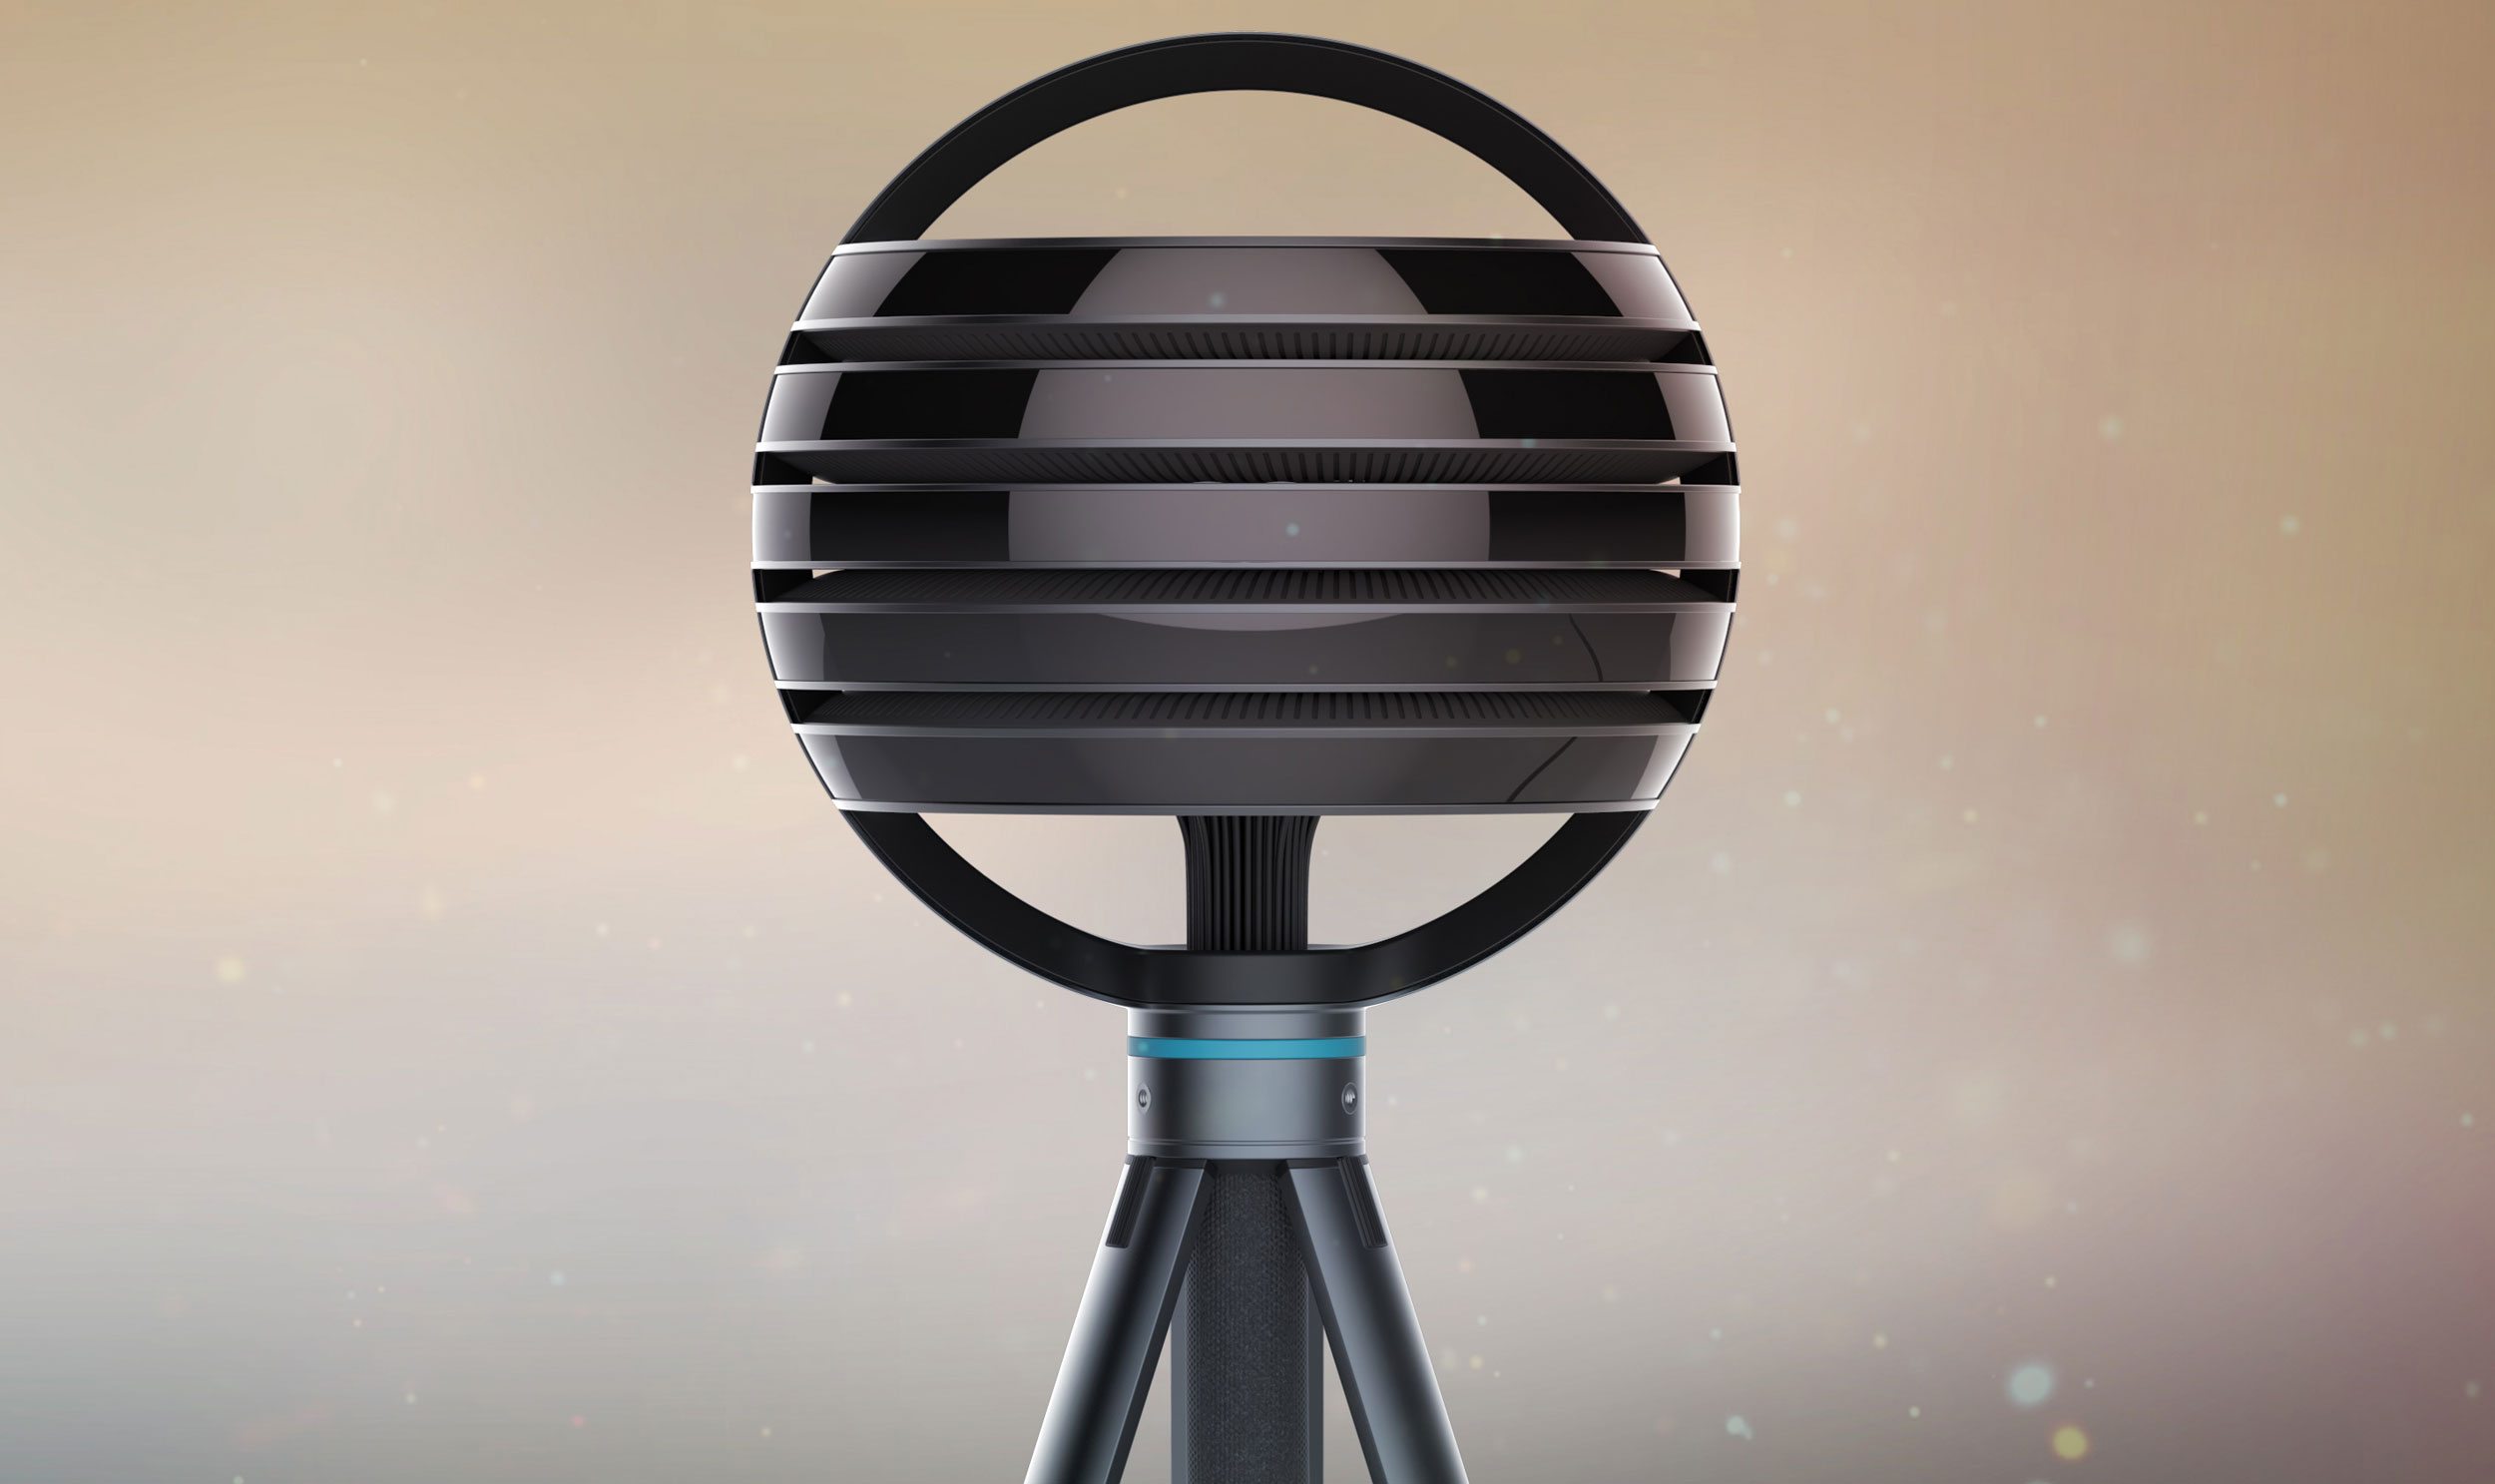
\includegraphics[scale=0.08]{lytro_immerge.jpg}
		\caption{the lytro immerge, designed to capture an entire scene at once, with an array of cameras built into the structure.}
		\label{fig:lytro_immerge}
	\end{minipage}\hfill
	\begin{minipage}{0.45\textwidth}
		\centering
		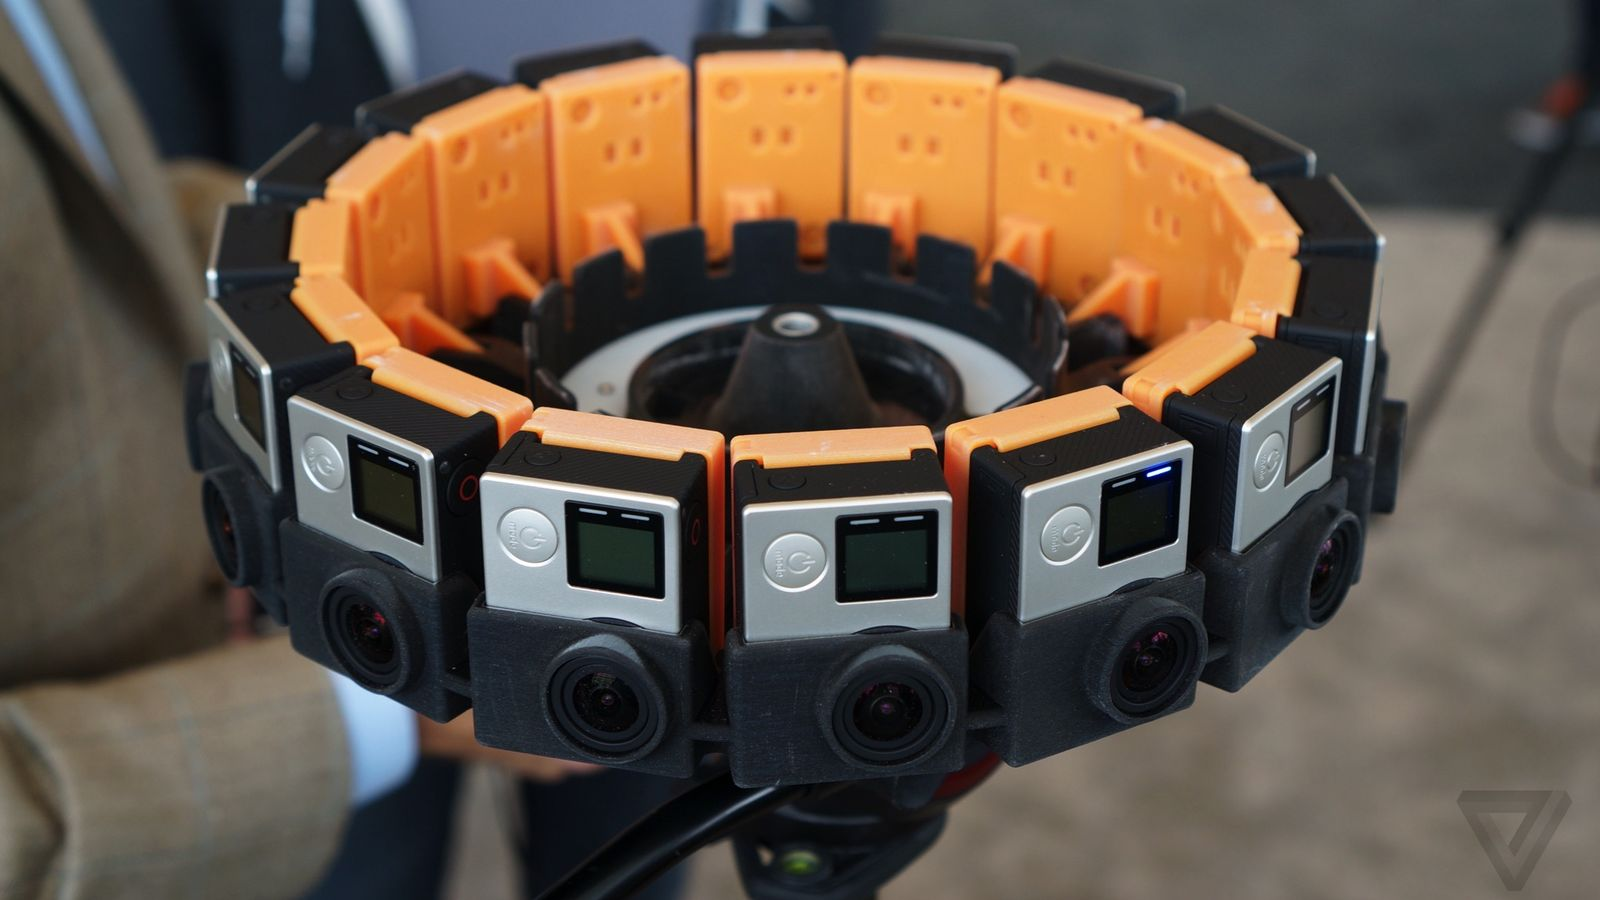
\includegraphics[scale=0.12]{jump_vr_video_cameras.jpg}
		\caption{On the right is the camera rig behind the Google Jump VR video system \cite{Anderson16}}
		\label{fig:jump_cameras}
	\end{minipage}
\end{figure}. 

As noted in the introduction, part of the goal of this project is to be able to collect light fields via cameras mounted on one or multiple multirotors, such as the one pictured in ***figure. The amount of research that has gone into multirotor navigation and use as a tool is substantial. A number of those papers were reviewed which could pertain to their use a light field collection devices, covering topics such as trajectory, localization, and data collection. 

In the first, the previously mentioned PTAM system is integrated into a new navigation system, allowing for fairly accurate localization of the multirotor \cite{Engel12}.

In another paper, the authors*** were interested in aircraft placement for optimum lighting effects in a scene... \cite{Srikanth14}

The final paper with In another, a system was developed to define the trajectory of a multirotor... \cite{Roberts16}



\chapter*{Progress to Date}
A considerable amount of work has been done so far in terms of learning, constructing light field viewers, and scratching at the limit of current state of the art techniques and technologies. This sections covers some of the hurdles in deducing what platforms to use, such as quantifying the accuracy of the systems involved, as well as collection, and finally on to intial rendering of acquired light fields.
\section*{Comparison of Platforms}
\section*{SLAM}
In the literature review section of this report, of interest is SLAM techniques. This will likely be key in determining the method by which 

\begin{figure}[!ht]
	\centering
	\includegraphics[scale=0.035]{mosaic.jpg}
	\caption{The plenoptic function at two points, showing all pencils of light rays \cite{Adelson91}}
	\label{fig:parameterization_visual}
\end{figure}

\begin{figure}[!ht]
	\centering
	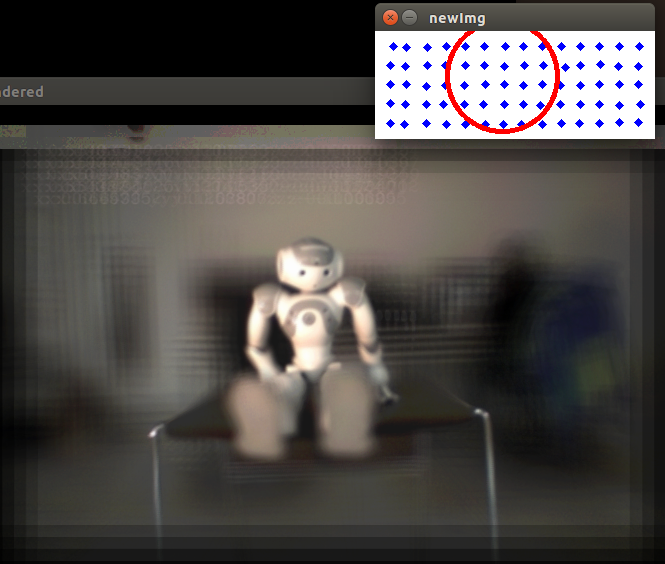
\includegraphics[scale=0.4]{nau_lf.png}
	\caption{The plenoptic function at two points, showing all pencils of light rays \cite{Adelson91}}
	\label{fig:parameterization_visual}
\end{figure}

\chapter*{Proposed Research}
\section*{steps}
Looking at the work utilizing SLAM in unstructured light fields and improving upon it by initially using the superior ORB-SLAM technique, then further by applying the methodology to 

PR2 image

Show ardrone image

While there are existing drones that can easily be controlled from the computer and capture data, there is clear lag high risk of data loss due to the transmission method (wifi). Instead, I would propose to make some simple modifications that would allow data capture and control in real time.
Drone Image + hardware

\section{First Step: Unstructured Light Fields with Robots}
First to replicate the experiment done with Davis, then with PR2 and Baxter, then on to drones.

\section{Second Step: Capturing Light Fields in Time}
The ability to allow a user to move through space and time could have huge implications in the realm of science and industry, allowing scietists to monitor experiments more closely than ever, and industry to monitor apparatus more in depth and with greater detail than before.

\begin{thebibliography}{10}%Any two digit number for more than nine references

\bibitem{Adelson91}
	Adelson, Edward H. (1991). \emph{The Plenoptic Function and Elements of Early Vision}

\bibitem{Anderson16}
	(2016). \emph{Jump: Virtual Reality Video}

\bibitem{Bolles87}
	(1987). \emph{Epipolar-Plane Image Analysis: An Approach to Determining Structure from Motion}

\bibitem{Chai00}
	(2000). \emph{Plenoptic Sampling}

\bibitem{Davis12}
	(2012). \emph{Unstructured Light Fields}

\bibitem{Engel12}
	(2012). \emph{Accurate Figure Flying with a Quadrocopter Using Onboard Visual and Intertial Sensing}

\bibitem{Gortler96}
	(1996). \emph{The Lumigraph}
	
\bibitem{Huang14}
	(2014). \emph{Light field modelling and interpolation using Kriging techniques}	
	
\bibitem{Ihrke16}
	(2016). \emph{Principles of Light Field Imaging}	
	
\bibitem{Isaksen01}
	(2001?). \emph{Dynamically Reparameterized Light Fields}

\bibitem{Jachnik13}
	(2013). \emph{Real-Time Surface Light-field Capture for Augmentation of Planar Specular Surfaces}
	
\bibitem{Joubert15}
	(2015). \emph{An Interactive Tool for Designing Quadrotor Camera Shots}

\bibitem{Kalantari16}
	(2016). \emph{Learning-Based View Synthesis for Light Field Cameras}

\bibitem{Katayama95}
	(1995). \emph{A Viewpoint Dependent Stereoscopic Display Using Interpolation of Multi-Viewpoint Images}
	
\bibitem{Kim13}
	(2013). \emph{Scene Reconstruction from High Spatio-Angular Resolution Light Fields}	
	
\bibitem{Klein07}
	(2007). \emph{Parallel Tracking and Mapping for Small AR Workspaces}	
	
\bibitem{Levoy96}
	(1996). \emph{Light Field Rendering}
	
\bibitem{Levoy06a}
	(2006). \emph{Light Fields and Computation Imaging}

\bibitem{Levoy06b}
	(2006). \emph{Light Field Microscopy}
	
\bibitem{McMillan95}
	(1995). \emph{Plenoptic Modelling: An Image-Based Rendering System}

\bibitem{Mur-Artal15}
	(2015). \emph{ORB-SLAM: a Versatile and Accurate Monocular SLAM System}

\bibitem{Ng06}
	(2006). \emph{Digital Light Field Photography}	

\bibitem{Oberlin16}
	(2016). \emph{Time-Lapse Light Field Photography With a 7 DoF Arm}

\bibitem{Roberts16}
	(2016). \emph{Generating Dynamically Feasible Drone Trajectories for Quadrotor Cameras}

\bibitem{Shi14}
	(2014). \emph{Light Field Reconstruction in the Continuous Fourier Domain}

\bibitem{Shum01}
	(2001). \emph{A Review of Image-based Rendering Techniques}

\bibitem{Srikanth14}
	(2014). \emph{Computational Rim Illumination with Aerial Robots}

\bibitem{Vaish06}
	(2006). \emph{Reconstructing Occluded Surfaces using Synthetic Apertures: Stero, Focus, and Robust Measures} 
	
\bibitem{Wilburn05}
	(2005). \emph{High-Speed Videography Using a Dense Camera Array}

stanford new light field archive http://lightfield.stanford.edu/

\end{thebibliography}

\end{document}